\label{Software architecture views}
\section{Software architecture views}
This chapter discuses the architecture of the system. It is first split into smaller parts and their dependencies on each other. The second paragraph describes the relation between hardware and software is explained. The third paragraph explains the data management. And the fourth paragraph describes the concurrency of the system.

\subsection{Subsystem decomposition}

The component diagram at \textbf{figure~\ref{fig:comp_diag}} shows the relations between the Tygron API, the connector and the GOAL agent. The GOAL agent has not been implemented yet, but will soon be. 

\begin{figure}[h]
	  \centering
	  \includegraphics[width=0.7\textwidth]{"Component diagram".pdf}
	  \caption{The component diagram}
	  \label{fig:comp_diag}
\end{figure}
This figure will show the different components the project uses and how they connect to each each other, however since we have not yet implemented anything, the goal agent is still empty. At this moment you can you just see how or non-existing bot will connect to the connector which in turn will connect to the Tygron API.

\subsection{Hardware/software mapping}
Our virtual human uses a different connection approach to the server than a real human user. When a session is created via the server, a user connects through its own client to that session. Our virtual human will connect to the session using a connector and the Tygron SDK. Visualisation of the actions performed by the virtual human are visible through a seperate instance of the Tygron Engine.

\begin{figure}
	\centering
	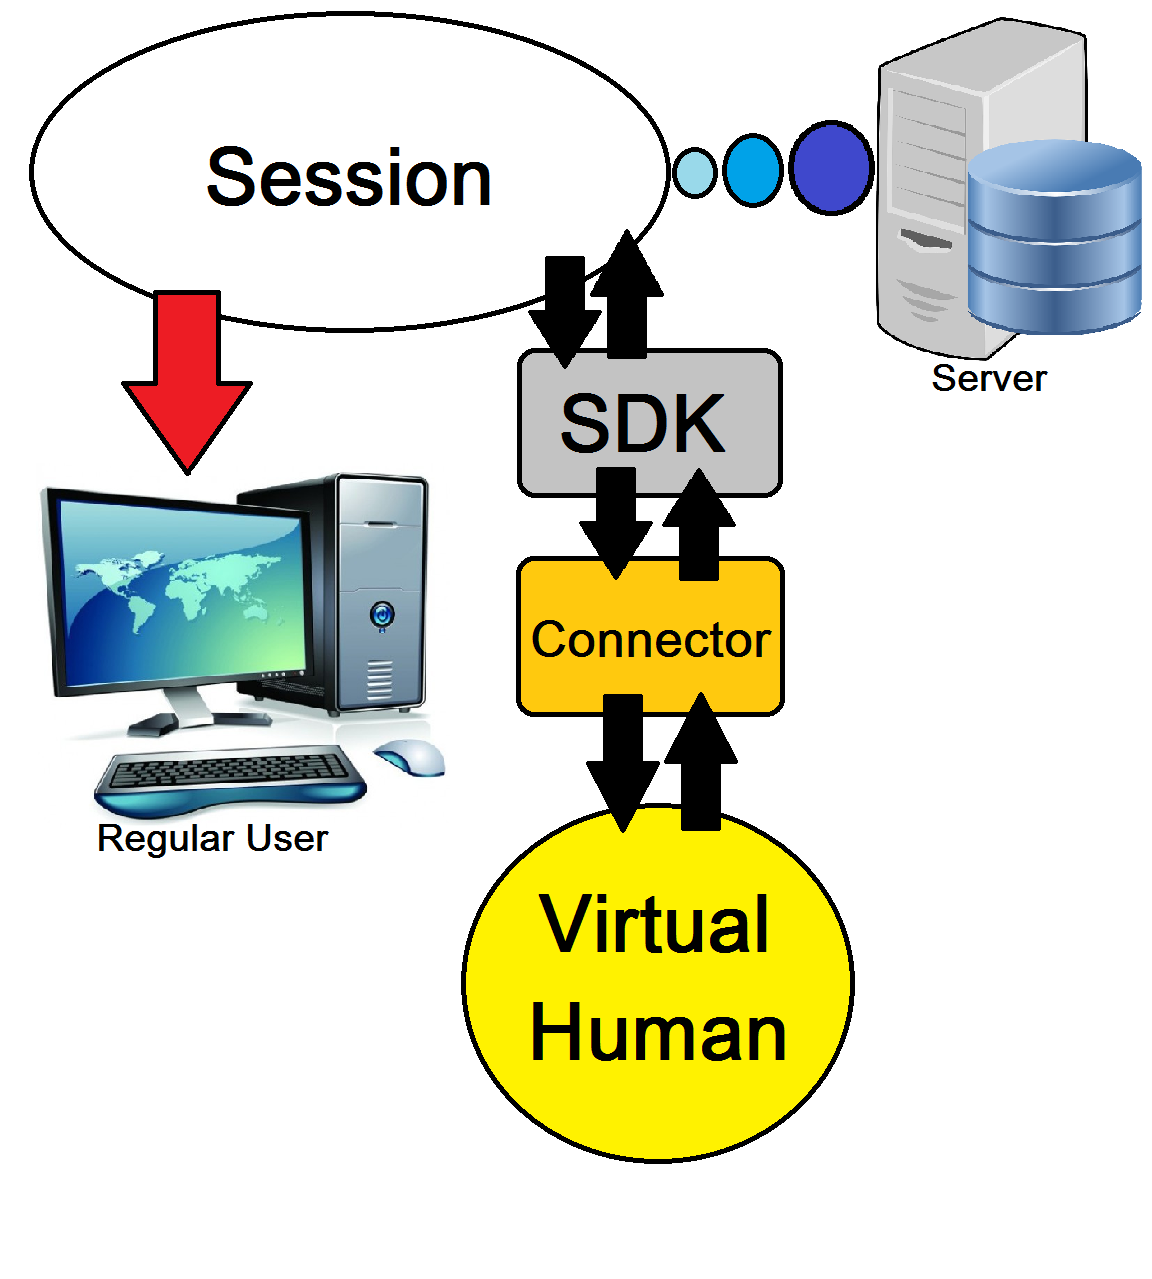
\includegraphics[width=0.7\textwidth]{Hardware_software_mapping}
	\caption{Hardware software mapping}
	\label{fig:Hard_soft_map}
\end{figure}

\subsection{Persistent data management}
Our GOAL agent is not responsible for storing persistent data, so it does not have external files or databases. This is so because everything is stored on the database of the Tygron server.
\subsection{Concurrency}
Our GOAL Agent is just one process. It shares recourses with other users of the Tygron environment. If a deadlock occurs, this would be on the Tygron environment. That is why our GOAL system won't have issues with deadlocks.
\newpage
